\chapter{Améliorations du développement logiciel}
    \section{Des outils de détection classique : quel point de départ ?}
        Comme vu en \ref{part2}, l'état de l'art en détection de vulnérabilités logicielles
        intègre déjà l'utilisation de LLM en aval de la phase de développement. Cette section
        propose une courte rétrospective des méthodes de détection de vulnérabilités classiques
        afin de mieux cerner la plus-value apportée par la détection en temps réel.
                \begin{figure}[H]
                    \centering
                    {\fbox{
                        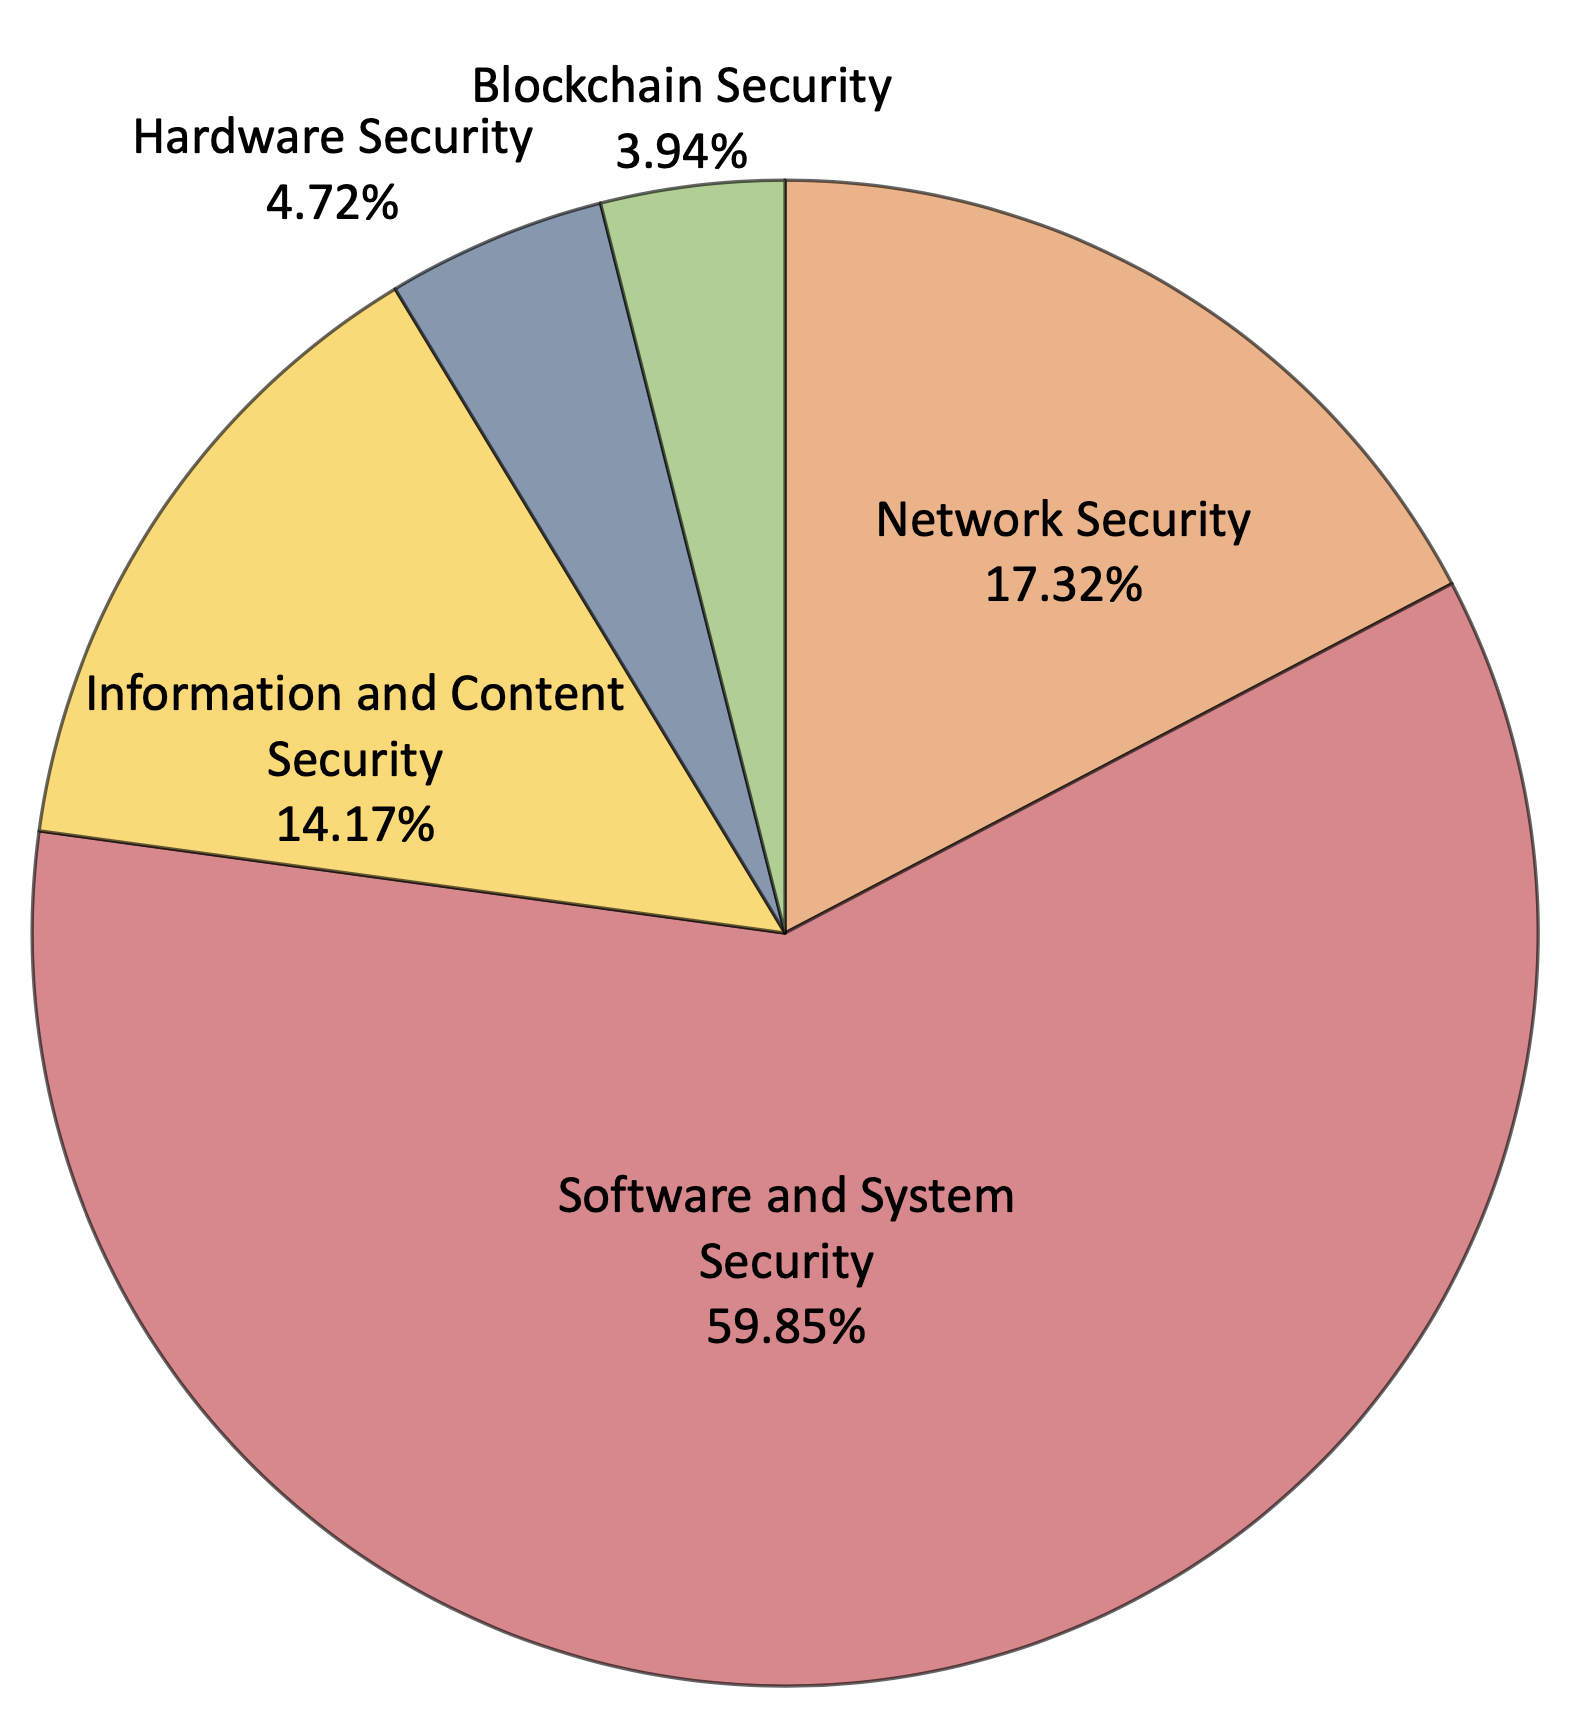
\includegraphics[width = 0.8\textwidth]{figures/Distribution of LLM usages in security domains}}}
                    \caption{Répartition de l'utilisation de LLM pour des tâches de sécurité\cite{citing4}}
                \end{figure}
        \newpage\subsection{Détection de vulnérabilités par IA : quelques outils à l'état de l'art}
            \subsubsection{Copilot}
                \texttt{Copilot} peut facilement être considéré comme le leader du développement
                assisté par LLM. Ses fonctionnalités sont nombreuses, bien éprouvées, et portées
                sur plusieurs modèles de pointe \textit{(GPT-4o, Claude 3.7 Sonnet ...)}.
                \texttt{Copilot} est désormais intégré sur de nombreux environnements de
                développement \textit{(VSCode, Suite Jetbrains ...)} et utilisé de façon quasi universelle.

                Par ailleurs, \texttt{Copilot} a servi de base de développement à un outil sorti
                en 2024 visant spécifiquement à introduire l'IA dans la cybersécurité : \texttt{Microsoft Copilot
                for Security }\footnote{https://www.youtube.com/watch?v=T3OKmtIPyzQ}. Si l'entreprise vante les
                mérites d'une analyse  évolutive en
                temps réel de l'outil\footnote{https://www.lemagit.fr/actualites/366621612/Microsoft-pousse-Security-Copilot-dans-lere-agentique}, la présente étude n'a pas trouvé de source
                mentionnant une capacité de celui-ci à détecter des vulnérabilités logicielles sur cette même
                temporalité. Cette feature est donc vraisemblablement absente ou méconnue des
                utilisateurs.
                \begin{figure}[H]
                    \centering
                    {\fbox{
                        \includegraphics[width = 0.8\textwidth]{figures/security-copilot-diagram}}}
                    \caption{Schéma conceptuel du fonctionnement de \texttt{Microsoft Copilot for Security}}
                \end{figure}
            \subsubsection{
\texttt{Snyk}, \textit{ powered by }
\texttt{Deepcode} : un exemple de standard industriel pour la sécurisation de code par IA}
                Cet outil permet de mener des analyses statiques de code à des fins spécifiques
                de sécurisation. Cependant, du propre aveu du développeur
                \footnote{https://docs.snyk.io/scan-with-snyk/snyk-code/manage-code-vulnerabilities/fix-code-vulnerabilities-automatically},
                l'outil ne propose pas systématiquement de correctif par peur de remplacer une
                vulnérabilité par une autre, ou de ne pas arriver à corriger celle identifiée.

                Par ailleurs, les analyses statiques ne permettent par définition pas à\texttt{Snyk} ne permet  pas de détecter les vulnérabilités en temps réel. Il est donc impossible d'utiliser cet outil pour corriger le code pendant la phase de développement.

        \subsection{Cas particulier du code généré par des LLM}
            Dans une perspective de nouveau paradigme de développement logiciel, il est
            important de considérer que le code revu par LLM peut également être un code généré
            par de tels modèles.

            \paragraph*{Pratiques actuelles de développement par LLM : exemple d'IntelliCode}
                Considéré comme le premier LLM développé pour générer du code \cite{citing3},
                \texttt{IntelliCode} est un outil moins récent que
                les deux
                précédemment
                cités \textit{(sa première publication académique datant de 2020\cite{IntelliCode})},
                mais encore largement utilisé, particulièrement dans la suite
                \texttt{Visual Studio}.

                La présente étude n'a pas trouvé de référence faisant explicitement part des
                aspects orientés sécurité de l'outil. Cette absence peut s'expliquer par la
                volonté de Microsoft de capitaliser sur les fonctionnalités plus récentes de \texttt{Microsoft Copilot
                for Security } pour en faire à terme un standard et laisser \texttt{IntelliCode}
                à son stade plus expérimentale.
    \section{Interprétation des métriques de classification présentées}\label{metriques}
            Les modèles présentés sont évalués selon les méthodes de Pearce et. Al \cite{38metrics},
        c'est-à-dire en se basant sur les scénarios prévus par le classement \texttt{MITRE} des 25
        vulnérabilités les plus importantes. En outre, ces scénarios prévoient une prévalence de
        certaines vulnérabilités \textit{(les injections SQL par exemple)}.

            Comme vu dans les parties précédentes, les métriques d'évaluation à proprement
        parler sont celles propres à un problème de classification, puisqu'il s'agit en
        l'occurrence d'une classification binaire 
\textit{(code vulnérable ou code non vulnérable)}. Les trois critères retenues sont la
précision, le rappel et le score F1. Leurs expressions sont rappelées ci-dessous :
        \begin{equation}
            \text{precision} = \frac{TP}{TP + FP} \;\;\;\; \text{rappel} = \frac{TP}{TP + FN} \;\;\;\; \text{score F1} = 2 \times \frac{\text{precision} \times \text{rappel}}{\text{precision} + \text{rappel}}
        \end{equation}

            Si ces métriques sont universelles et facilement interprétables, celles-ci sont
            parfois insuffisantes pour évaluer finement la performance d'un modèle de
            classification. C'est d'ailleurs ce qui est rappelé dans l'article cité dans la partie
            sur les métriques d'évaluation \cite{40article}. Celui-ci propose de compléter les
            trois critères cités précédemment par des métriques moins triviales et moins
            biaisées au sens de l'auteur.

    \section{Correction et complétion pendant la phase de développement : promesses et difficultés rencontrées}
        Les parties précédentes montrent que la détection de vulnérabilités en temps réel est
        grandement améliorée par les LLM développés, en particulier \texttt{CodeBERT} fine-tuné.
        Cette conclusion est valable pour le code généré par IA comme pour le code "strictement
        humain".

        À la lumière des sections de ce chapitre, on peut affirmer que ces résultats sont
        prometteurs pour le secteur du développement logiciel, la correction par LLM lors de la
        phase de développement n'ayant été proposée par aucun outil à l'état de l'art.

        On relève cependant plusieurs points d'amélioration notables : aucun outil de
        développement par LLM n'est actuellement sensiblement meilleur que ses concurrents \textit{(sur les aspects de sécurité mais pas exclusivement)}, ne
        laissant pas la possibilité à court de terme de voir la naissance d'un nouveau standard.
        Par ailleurs, les LLM présentés ici nécessitent vraisemblablement plusieurs autres
        phases d'évaluation plus poussées avant un déploiement industriel. Ces remarques
        serviront de point de départ pour le prochain chapitre.